\documentclass[tikz]{standalone}

\usetikzlibrary{shapes.geometric, arrows, calc}
\tikzstyle{startstop} = [rectangle, rounded corners, minimum width=3cm, minimum height=1cm, text centered, draw=black] % fill=red!30
\tikzstyle{io} = [trapezium, trapezium left angle=70, trapezium right angle=110, minimum width=3cm, minimum height=1cm, text centered, draw=black] % fill=blue!30
\tikzstyle{process} = [rectangle, minimum width=3cm, minimum height=1cm, text centered, text width=3cm, draw=black] % fill=orange!30
\tikzstyle{decision} = [diamond, minimum width=2cm, minimum height=1cm, text centered, draw=black, text width=3cm] % fill=green!30
\tikzstyle{arrow} = [thick,->,>=stealth]

\begin{document}
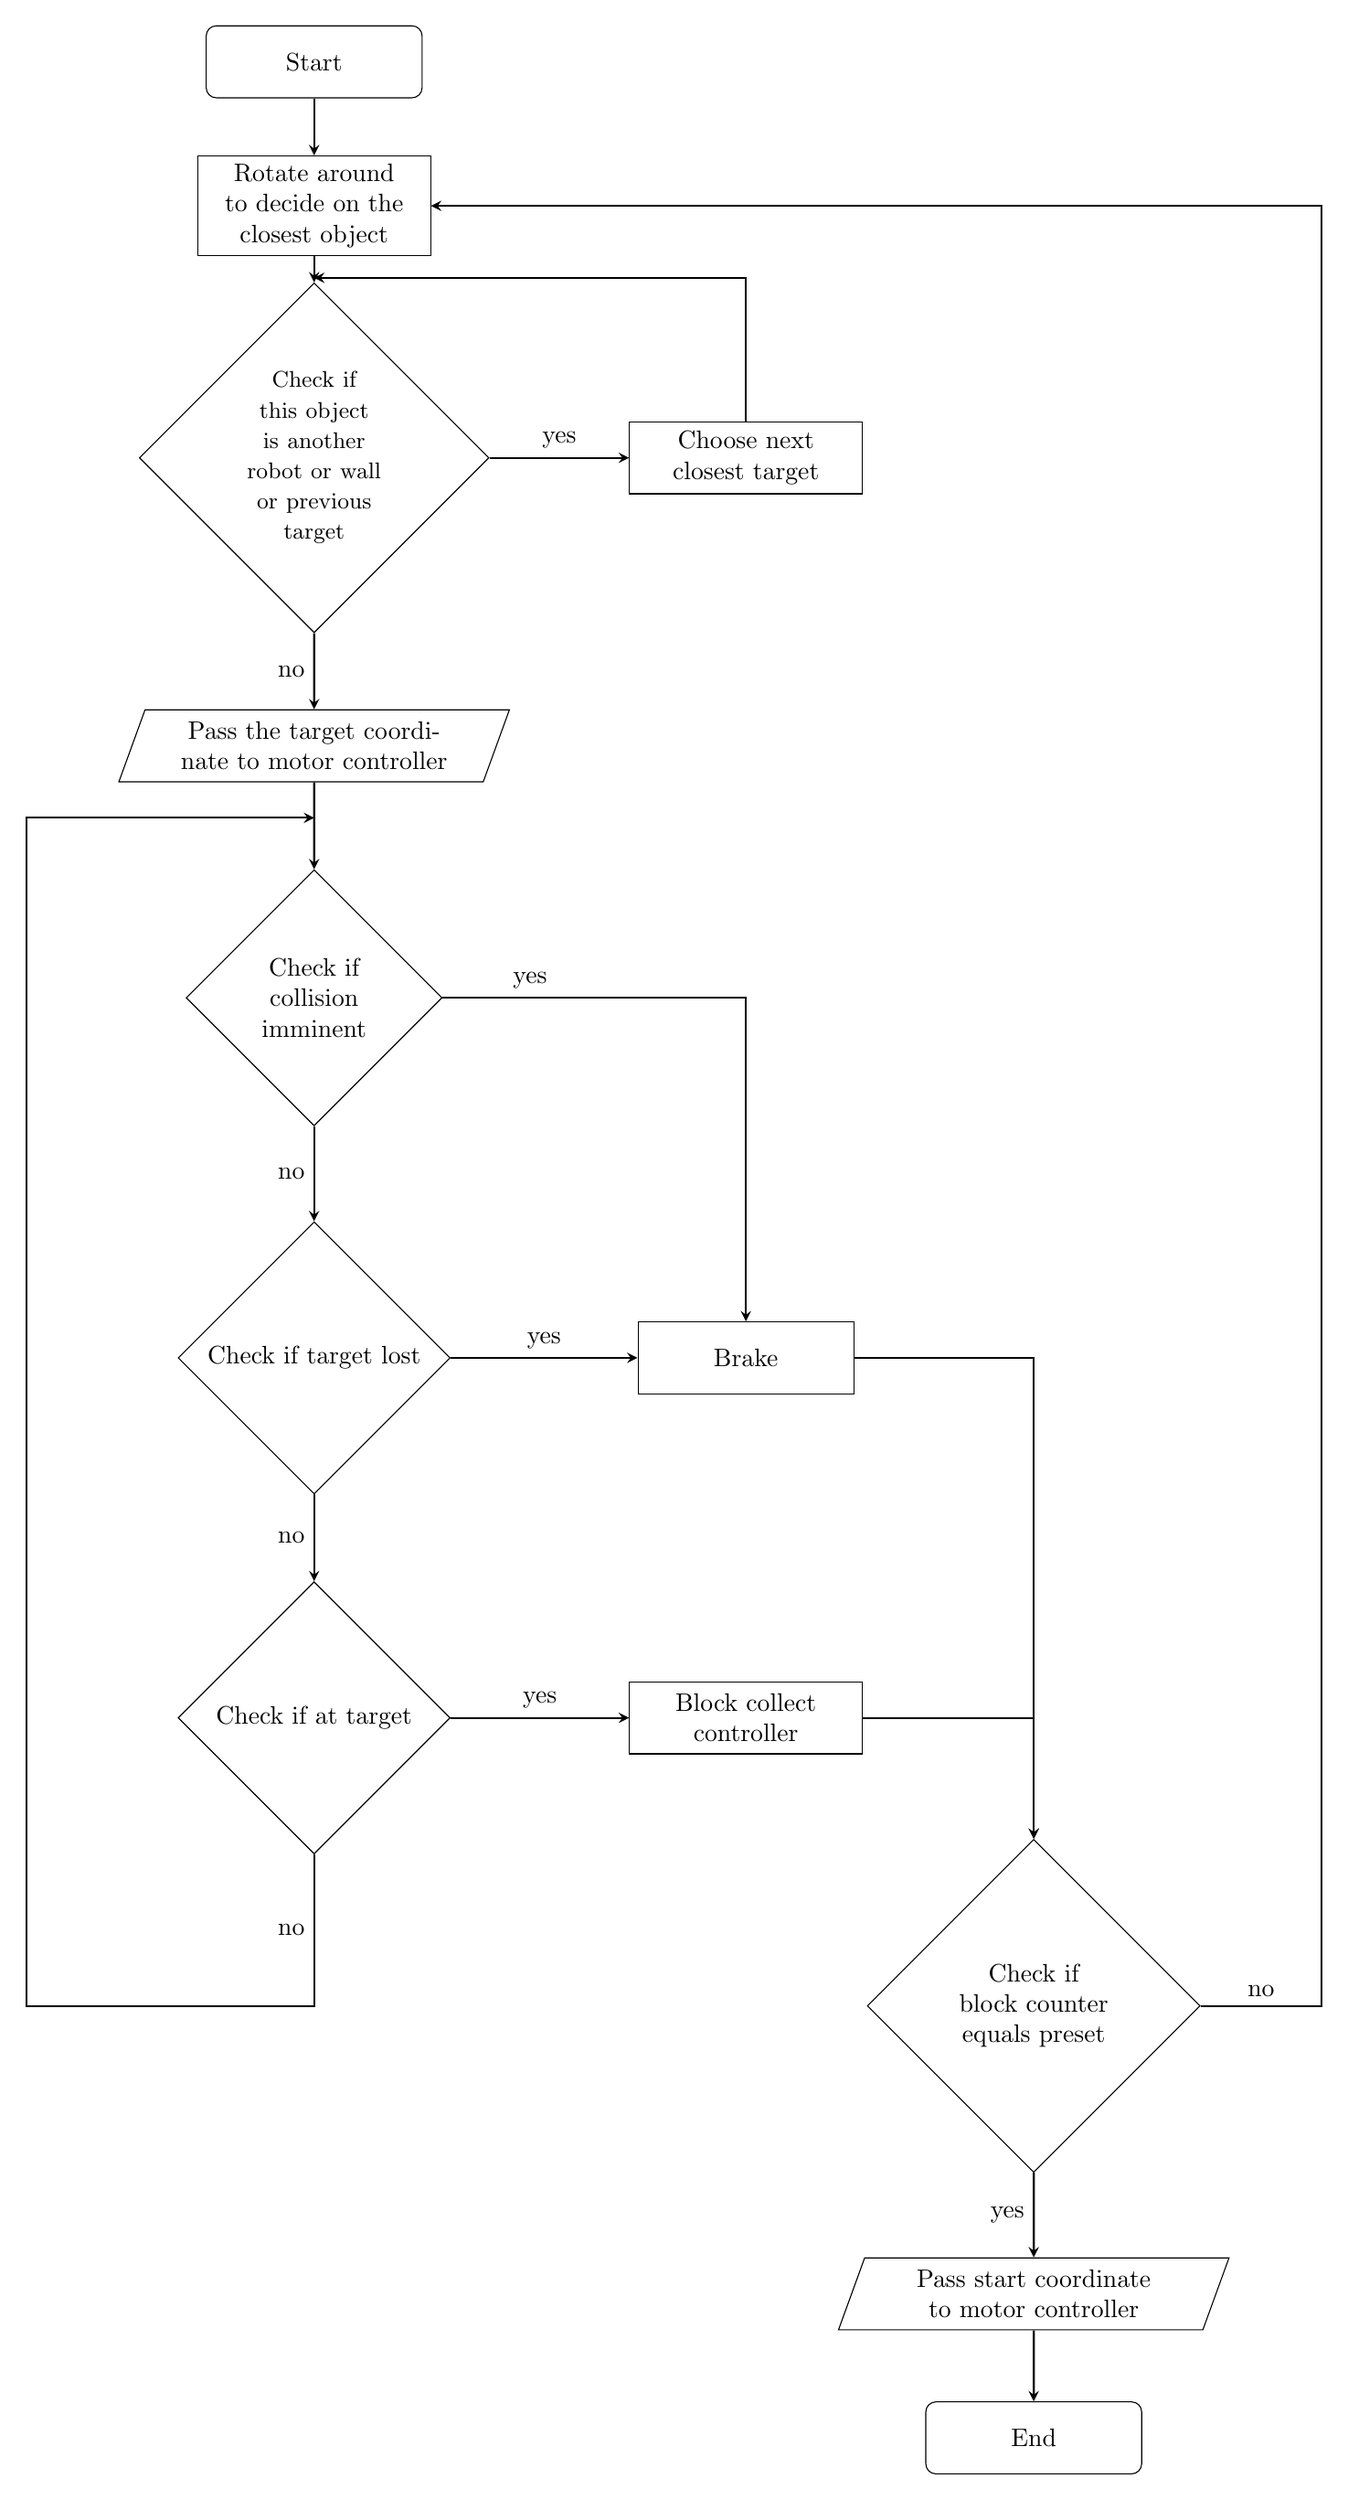
\begin{tikzpicture}[node distance=2cm]
\node (start) [startstop] {Start};

\node (rotate) [process, below of=start] {Rotate around to decide on the closest object};

\node (check_obj) [decision, below of=rotate, yshift=-1.5cm, text width=2cm] {\small Check if this object is another robot or wall or previous target};

\node (no1) [io, below of=check_obj, yshift=-2cm, text width=4cm] {Pass the target coordinate to motor controller};
\node (yes1) [process, right of=check_obj, xshift=4cm] {Choose next closest target};

\node (check_collision) [decision, below of=no1, yshift=-1.5cm, text width=2cm] {Check if collision imminent};


\node (check_target_loss) [decision, below of=check_collision, yshift=-3cm] {Check if target lost};

\node (brake) [process, right of=check_target_loss, xshift=4cm, text width=1cm] {Brake};

\node (check_at_target) [decision, below of=check_target_loss, yshift=-3cm] {Check if at target};

\node (collect) [process, right of=check_at_target, xshift=4cm] {Block collect controller};


\node (check_num) [decision, below of=collect, xshift=4cm, yshift=-2cm] {Check if block counter equals preset};

\node (home) [io, below of=check_num, yshift=-2cm, text width=4cm] {Pass start coordinate to motor controller};

\node (end) [startstop, below of=home] {End};


\draw [arrow] (start) -- (rotate);
\draw [arrow] (rotate) -- (check_obj);

\draw [arrow] (check_obj) -- node[left] {no} (no1);
\draw [arrow] (check_obj) -- node[above] {yes} (yes1);
\draw [arrow] (yes1) |- (0, -3cm);

\draw [arrow] (no1) -- (check_collision);

\draw [arrow] (check_collision) -- node[left]{no} (check_target_loss);
\draw [arrow] (check_target_loss) -- node[above] {yes} (brake);
\draw [arrow] (check_collision) -| node[above, xshift=-3cm] {yes} (brake);

\draw [arrow] (check_target_loss) -- node[left]{no} (check_at_target);
\draw [arrow] (check_at_target) -- node[above] {yes} (collect);
\draw [arrow] (check_at_target) -- node[left]{no} ++(0, -4cm) -- ++(-4cm, 0) |- ($ (check_collision) + (0, 2.5cm) $);

\draw [arrow] (brake) -| (check_num);
\draw [arrow] (collect) -| (check_num);

\draw [arrow] (check_num) -- node[above]{no} ++(4cm, 0) |- (rotate);
\draw [arrow] (check_num) -- node[left] {yes} (home);
\draw [arrow] (home) -- (end);

\end{tikzpicture}
\end{document}
